\newpage{\pagestyle{empty}\cleardoublepage}
\newpage
\vspace*{\fill}
    \begin{center}
      \thispagestyle{empty} \vspace*{0cm} \textbf{\huge
Manual de Usuario}
    \end{center}
    \vspace*{\fill}
\newpage{\pagestyle{empty}\cleardoublepage}
\chapter{Manual de Usuario}

Antes de entrar en cada uno de los usuarios cabe mencionar las diferentes vistas comunes o formatos seguidos en las p\'{a}ginas y eventos comunes.

\begin{enumerate}
\item Cargador de Progreso. Este modal bloquear\'{a} la p\'{a}gina cuando alg\'{u}n tipo de carga as\'{i}ncrona est\'{e} en uso.
\begin{figure}[h!]
\centering

\includegraphics[width=.3\textwidth]{Img/ManualUsuario/PROGRESS_SPINNER.png}
\end{figure}
\item Verificaciones o preguntas de '`? Est\'{a}s seguro?'
\begin{figure}[h!]
\centering
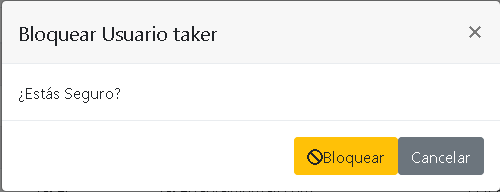
\includegraphics[width=.6\textwidth]{Img/ManualUsuario/ADMIN_BLOCK_USER.png}
\end{figure}
\end{enumerate}


\section{Usuario no logueado}
\subsection{P\'{a}gina Principal}
De ahora en adelante GUEST, el usuario no logueado dispondr\'{a} de la misma vista principal que los usuarios del sistema, salvo el men\'{u} de navegaci\'{o}n, el cual mostrar\'{a} opciones extra a los usuarios que inicien sesi\'{o}n.\\

\begin{figure}[h!]
\centering
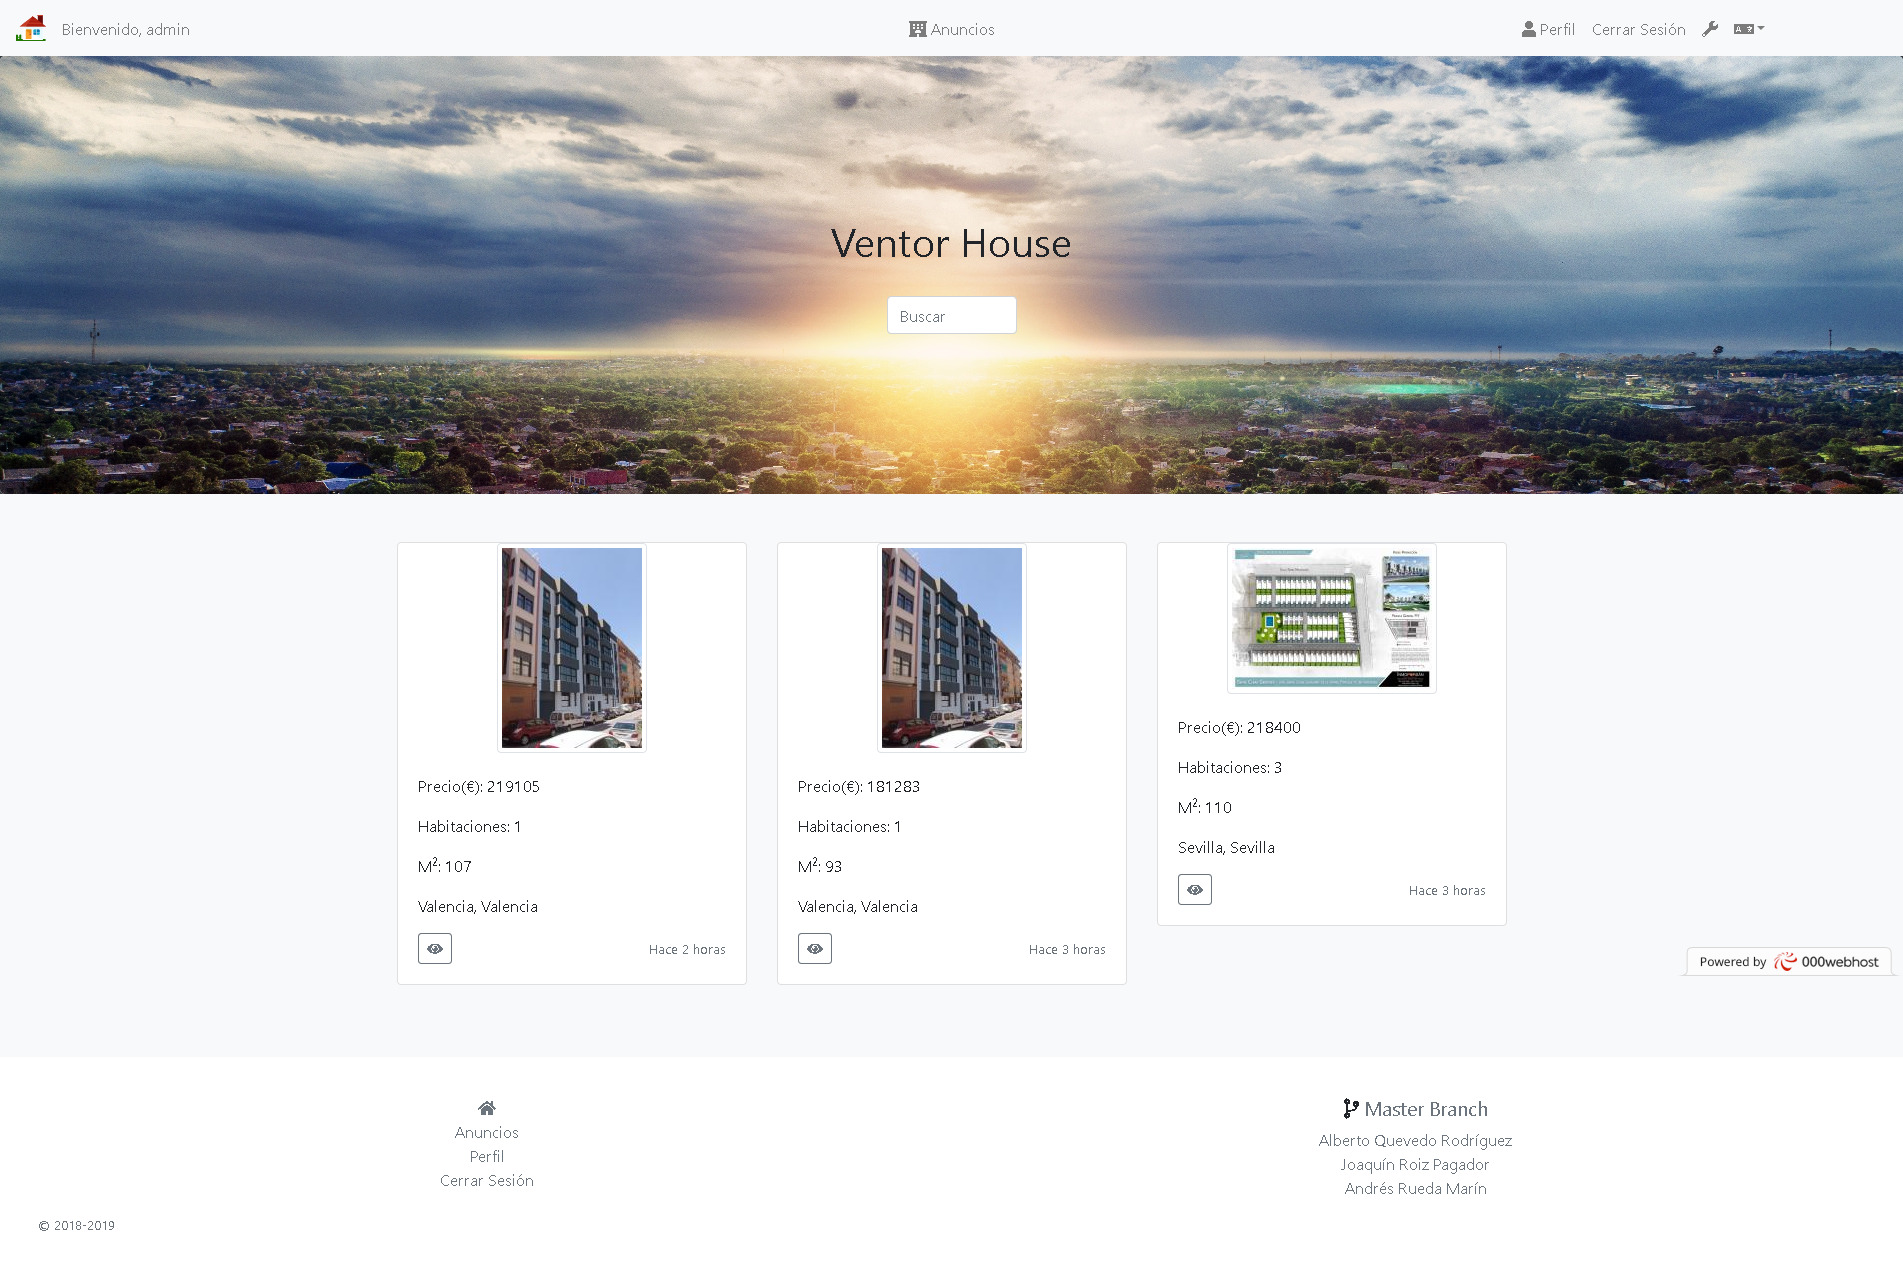
\includegraphics[width=.7\textwidth]{Img/ManualUsuario/PPAL_GUEST.jpg}
\end{figure}

En primer lugar se puede observar una barra de navegaci\'{o}n, en la cual se aprecia una imagen de una casa. Si se hace click en ella, se llevar\'{a} a esta p\'{a}gina principal. En la zona central del men\'{u} se encuentra el acceso al listado de todos los anuncios del sistema, para poder listarlos y filtrarlos correctamente. Tras esto, la opci\'{o} de iniciar sesi\'{o}n y un desplegable que ofrecer\'{a} un cambio de idioma, entre espa\~{n}ol e ingl\'{e}s.

\begin{figure}[h!]
\centering

\includegraphics[width=1\textwidth]{Img/ManualUsuario/NAV_GUEST.png}
\end{figure}


En la parte superior de la p\'{a}gina principal, el usuario GUEST podr\'{a} realizar una b\'{u}squeda global escribiendo las palabras claves por las que quiere buscar, y se le listar\'{a} un m\'{a}ximo de 10 resultados en tiempo real. Al seleccionar uno de los anuncios se acceder\'{a} a su respectiva vista, donde se podr\'{a} consultar todo dato relacionado con el mismo, as\'{i} como ver sus fotos detenidamente.

\begin{figure}[h!]
\centering
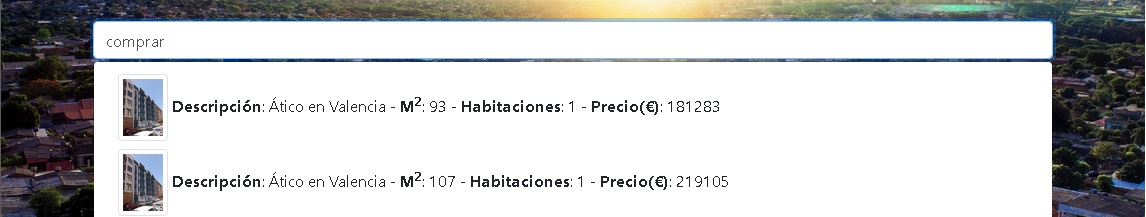
\includegraphics[width=0.7\textwidth]{Img/ManualUsuario/GLOBAL_SEARCH_GUEST.jpg}
\end{figure}


En caso de que el usuario GUEST decida pulsar intro al escribir las palabras claves en el buscador, se le redirigir\'{a} a la siguiente p\'{a}gina con una b\'{u}squeda global paginada, en la cual se podr\'{a}n ver tarjetitas con los anuncios resultantes de la b\'{u}squeda.

\begin{figure}[h!]
\centering
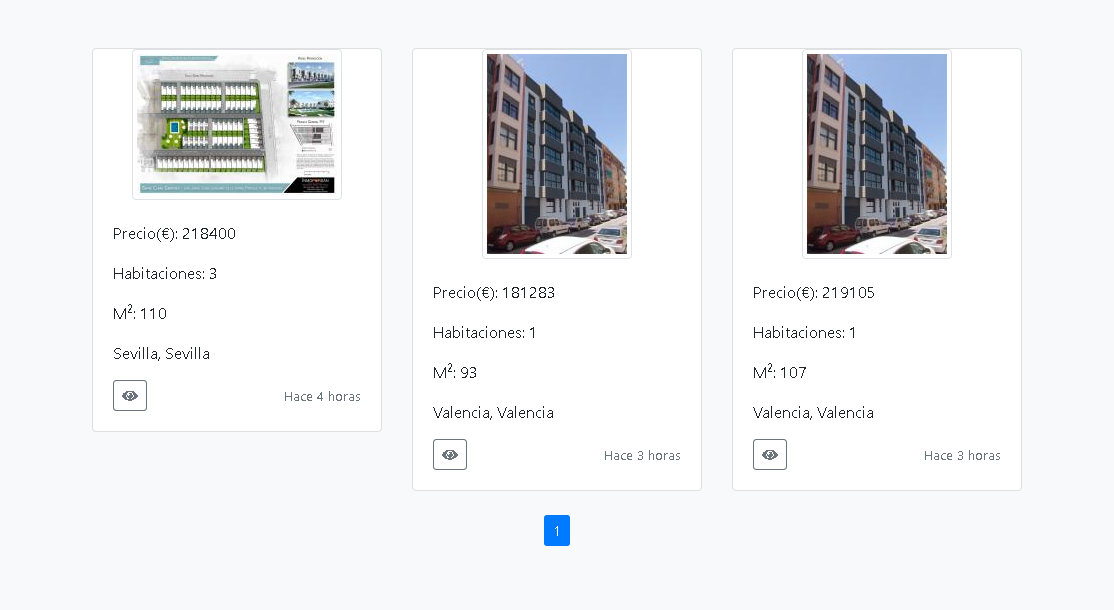
\includegraphics[width=.7\textwidth]{Img/ManualUsuario/GLOBAL_SEARCH_ENTER.png}
\end{figure}

Siguiendo en la p\'{a}gina principal, debajo del buscador existente se encuentran listadas 9 tarjetas con los \'{u}ltimos anuncios creados en el sistema, donde el usuario por\'{a} seleccionar alguna y acceder a la p\'{a}gina del anuncio en cuesti\'{o}n.


\begin{figure}[h!]
\centering
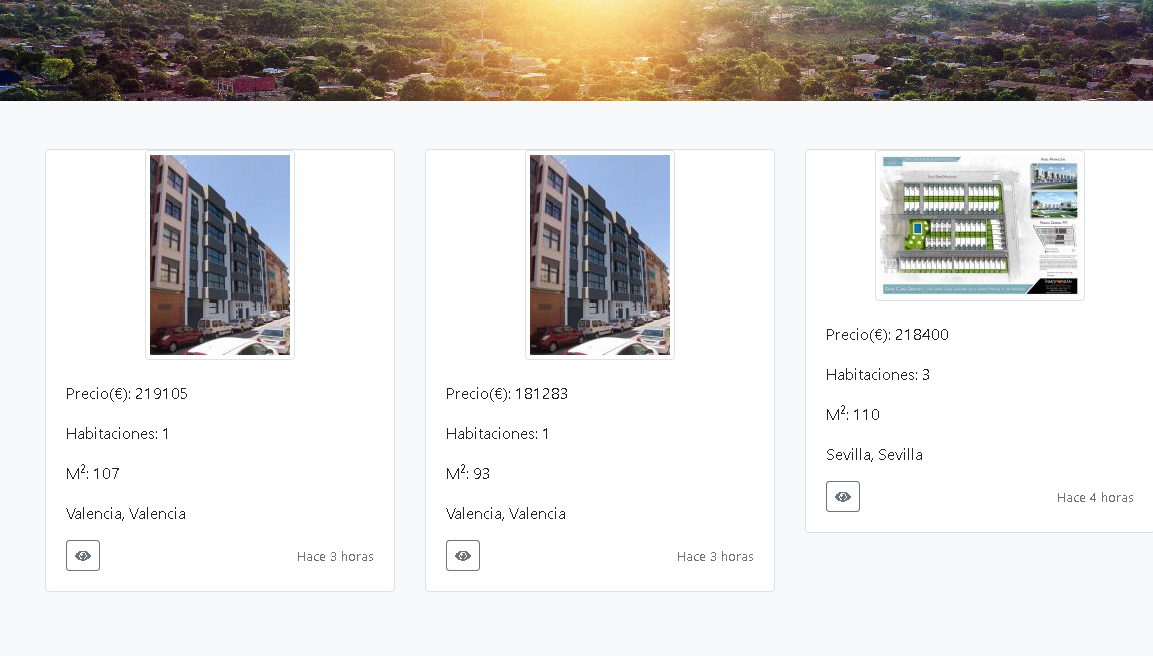
\includegraphics[width=.5\textwidth]{Img/ManualUsuario/TARJETAS.png}
\end{figure}


Debajo de estas tarjetas, y com\'{u}n a todas las p\'{a}ginas se puede encontrar un footer con la informaci\'{o}n de los desarrolladores, as\'{i} como algunos links interesantes para facilitar la navegaci\'{o}n del usuario desde abajo.

\begin{figure}[h!]
\centering

\includegraphics[width=1\textwidth]{Img/ManualUsuario/FOOTER.png}
\end{figure}

\subsection{Registro e Inicio de Sesi\'{o}n}
En la pantalla de inicio de sesi\'{o}n se puede encontrar un formulario sencillo que solicita las credenciales para entrar en el sistema. Con usuario o email y la contrase\~{n}a adecuados, el usuario podr\'{a} identificarse en el sistema y acceder a las dem\'{a}s opciones del mismo.


\begin{figure}[h!]
\centering

\includegraphics[width=.7\textwidth]{Img/ManualUsuario/LOGIN.png}
\end{figure}


Para poder iniciar sesi\'{o}n, el usuario GUEST deber\'{a} registrarse, haciendo click en la pesta\~{n}a con el t\'{i}tulo 'Registro'. En \'{e}sta, se le ofrecer\'{a} un formulario con 7 campos, los cuales solicitan nombre, apellidos, email, tel\'{e}fono, login y contrase\~{n}a (dos veces para verificar).

\begin{figure}[h!]
\centering
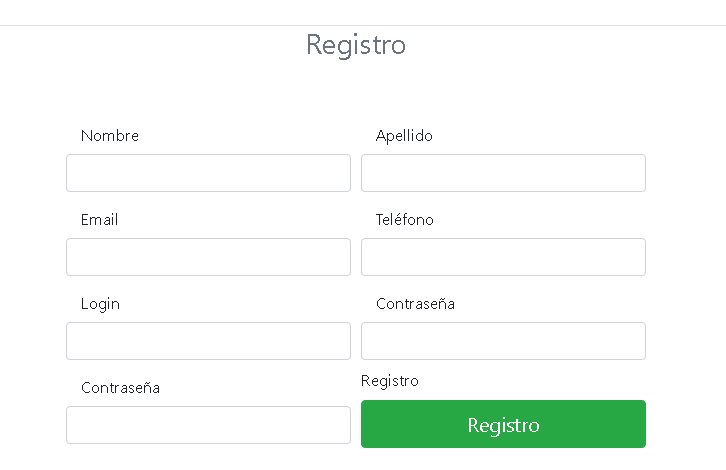
\includegraphics[width=.5\textwidth]{Img/ManualUsuario/REGISTRO.png}
\end{figure}

En caso de existir alg\'{u}n fallo en alguno de estos formularios, se le mostrar\'{a} al usuario un mensaje con el formato similar al siguiente:

\begin{figure}[h!]
\centering

\includegraphics[width=.3\textwidth]{Img/ManualUsuario/ERROR_LOGIN.png}
\end{figure}


\subsection{Anuncios}
Habiendo accedido a la secci\'{o}n del men\'{u} con el t\'{i}tulo 'Anuncios', se presenta una p\'{a}gina con un men\'{u} a la izquierda que permite filtrar los resultados mostrados en funci\'{o}n del tipo de operaci\'{o}n y el tipo de casa. Del mismo modo, los resultados se mostrar\'{a}n paginados, de forma que se podr\'{a} navegar entre los muchos anuncios que puedan coincidir con el criterio de filtro aplicado.

\begin{figure}[h!]
\centering
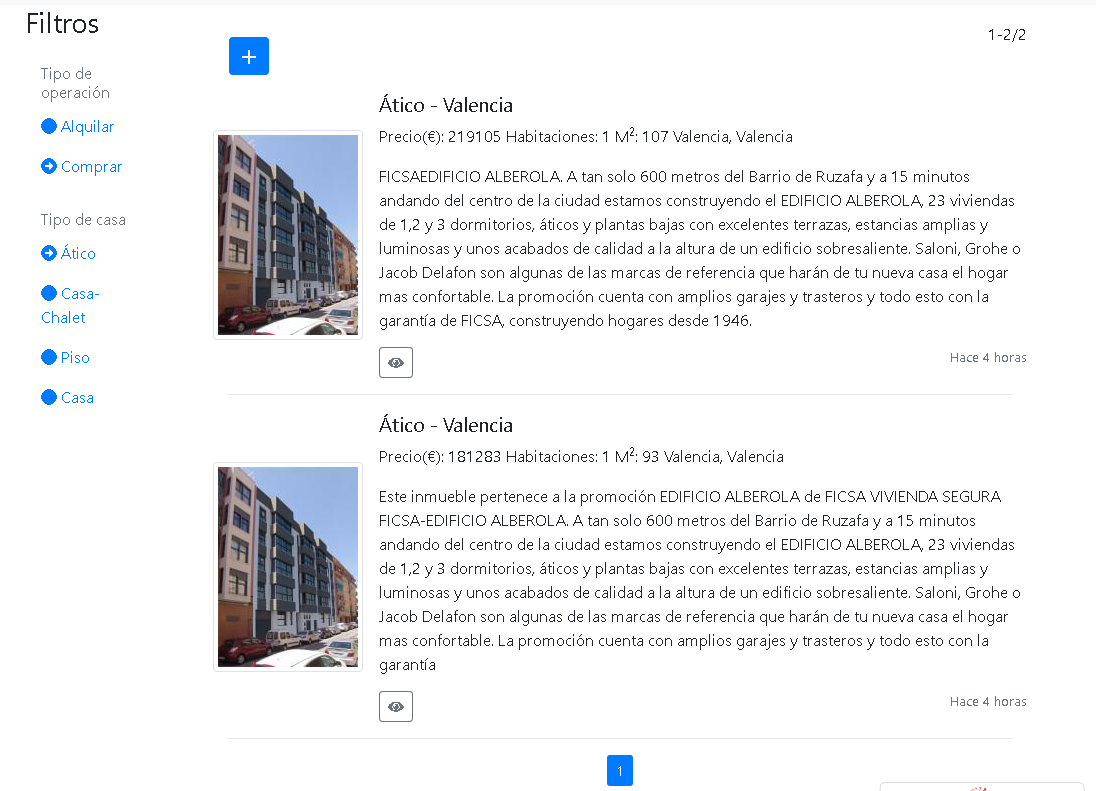
\includegraphics[width=.7\textwidth]{Img/ManualUsuario/LISTADO_ANUNCIOS.png}
\end{figure}


Al hacer click en un ad se apreciar\'{a} el siguiente contenido:

\begin{figure}[h!]
\centering
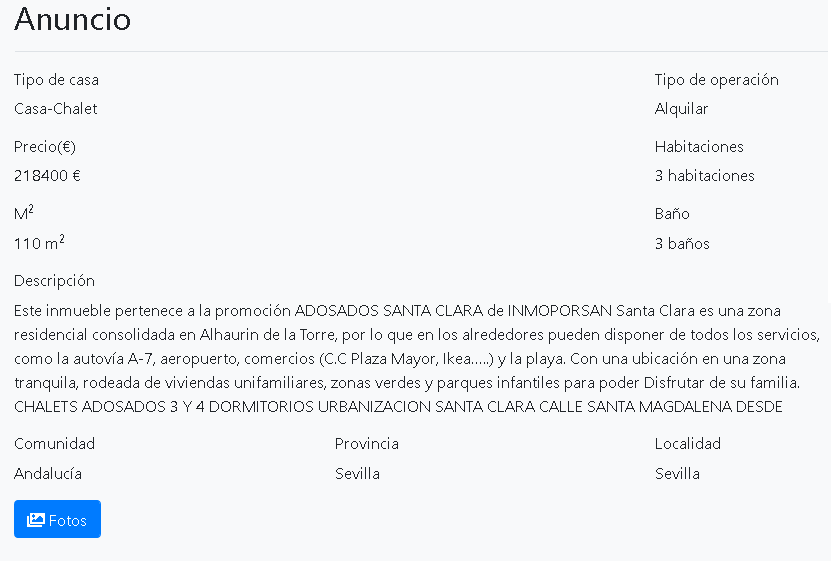
\includegraphics[width=.7\textwidth]{Img/ManualUsuario/ANUNCIO_GUEST.png}
\end{figure}

De un anuncio se obserar\'{a} el tipo de vivienda, tipo de operaci\'{o}n, precio, habitaciones, metros cuadrados, n\'{u}mero de ba\~{n}os, su descripci\'{o}n y los datos referentes a su localizaci\'{o}n geogr\'{a}fica.\\

A la derecha de estos, encontrar\'{a} un men\'{u} con el nombre del anunciante y las acciones posibles a realizar sobre el anuncio en cuesti\'{o}n. Para el usuario GUEST, la apariencia ser\'{a} como la que sigue:

\begin{figure}[h!]
\centering
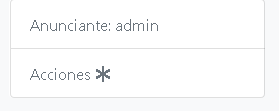
\includegraphics[width=.3\textwidth]{Img/ManualUsuario/LAGERAL_AD_GUEST.png}
\end{figure}

Para poder realizar m\'{a}s opciones, sere\'{a} recomendable iniciar sesi\'{o}n, dado que las operaciones ofrecidas son personalizadas al usuario registrado en el sistema.\\

Debajo del propio anuncio y sus datos se encuentra el bot\'{o}n 'Fotos', con el contenido de las im\'{a}genes, el cual no aparecer\'{a} si el anuncio no dispone de las mismas. Al hacer click sobre \'{e}l, se abrir\'{a} una ventana modal con la galer\'{i}a de im\'{a}genes asociadas al anuncio, navegables de forma lateral y con la posibilidad de hacer zoom en cada imagen al hacer click en ellas.

\begin{figure}[h!]
\centering
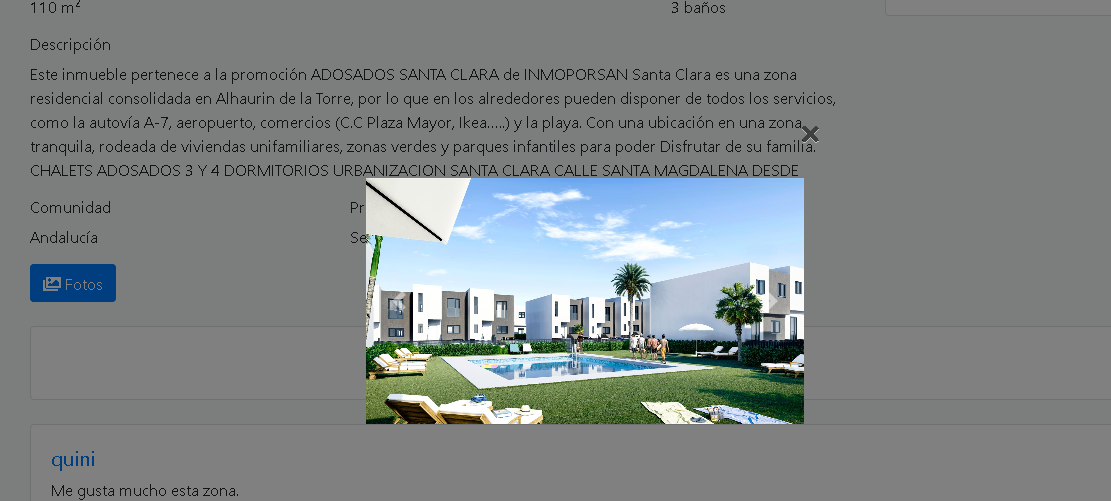
\includegraphics[width=.7\textwidth]{Img/ManualUsuario/GALERIA_GUEST.png}
\end{figure}

Por \'{u}ltimo, bajo esta secci\'{o}n, podr\'{a} encontrar una solicitud de iniciar sesi\'{o}n para poder comentar, seguida de un listado de comentarios, siendo el m\'{a}s reciente el que aparezca en la parte superior. Se podr\'{a}n paginar a partir del bot\'{o}n inferior facilitado para ello.

\begin{figure}[h!]
\centering
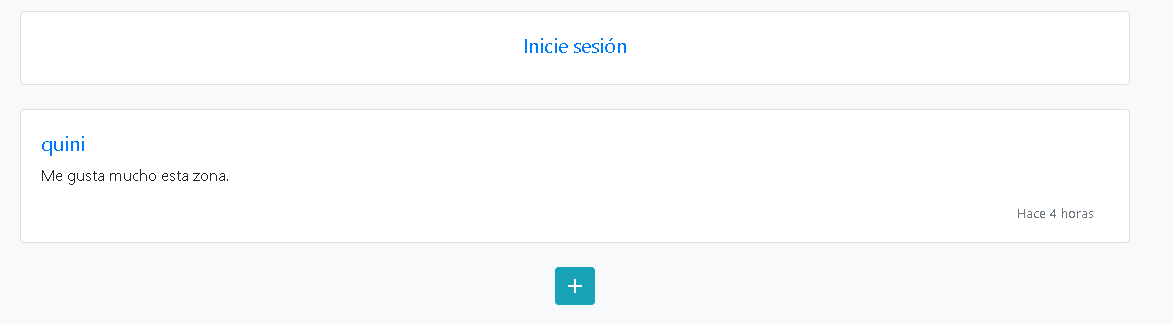
\includegraphics[width=.7\textwidth]{Img/ManualUsuario/COMENTARIOS_GUEST.png}
\end{figure}